\documentclass[11pt,pdf,aspectratio=43]{beamer}
\usepackage[utf8]{inputenc}
\usepackage[russian]{babel}
\usepackage[T2A]{fontenc}
\usepackage{movie15}
\usepackage{wrapfig}
\graphicspath{video/}
\usetheme{Boadilla}
\usefonttheme{structurebold}
\usefonttheme[onlymath]{serif}
\setbeamercovered{transparent}

\title[]{Мультистационарные системы. Биологический триггер с сосредоточенными 
параметрами.}
\date[]{}

\begin{document}

\begin{frame}[plain]
\maketitle
\end{frame}

\section{Биологический триггер}
\begin{frame}
	\frametitle{Синтез фермента и катализируемого продукта}
	\begin{wrapfigure}[9]{l}{0.5\textwidth}
		\vspace{-5ex}
		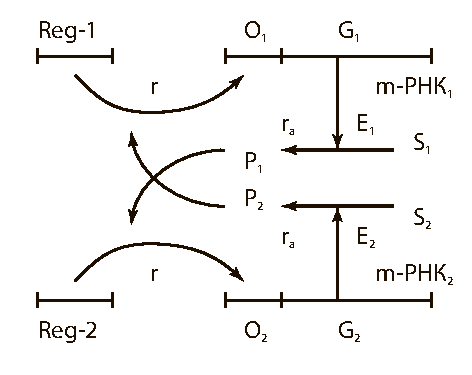
\includegraphics[width=0.5\textwidth]{images/jacob_mono}
	\end{wrapfigure}
	\[
	    \left\{ \begin{array}{ll}
	        \cfrac{dE}{dt} = \cfrac{1}{\tau_E}I - \cfrac{1}{\tau_2}E \\
	        \cfrac{dP}{dt} = E\cfrac{k_{+2}S}{K_S + S} - qP \\
	        \cfrac{dI}{dt} = Q(r) - \cfrac{1}{\tau_1}I
	    \end{array} \right.
	\]
\end{frame}
\begin{frame}
	\frametitle{Триггерная схема Жакоба-Моно}
	\[
		\left\{ \begin{array}{ll}
	        \cfrac{dx_1}{dt} = \cfrac{L_1}{1+\gamma x_2^m} - x_1 \\
	        \cfrac{dx_2}{dt} = \cfrac{L_2}{1+\gamma^{-1} x_1^m} - x_2  
	    \end{array} \right.
    \]
\end{frame}
\begin{frame}
	\frametitle{Исследование триггерной системы}
	\[
		\left\{ \begin{array}{ll}
	        \cfrac{dx_1}{dt} = \cfrac{L_1}{1+\gamma x_2^2} - x_1 \\
	        \cfrac{dx_2}{dt} = \cfrac{L_2}{1+\gamma^{-1} x_1^2} - x_2  
	    \end{array} \right.
	\]
\end{frame}

\end{document}
